%\addcontentsline{toc}{chapter}{Development Process}
\chapter{Design}

\section{Overall Architecture}

\subsection{Class Descriptions}
\subsubsection{Game Classes}
\begin{figure}[h]
\centering
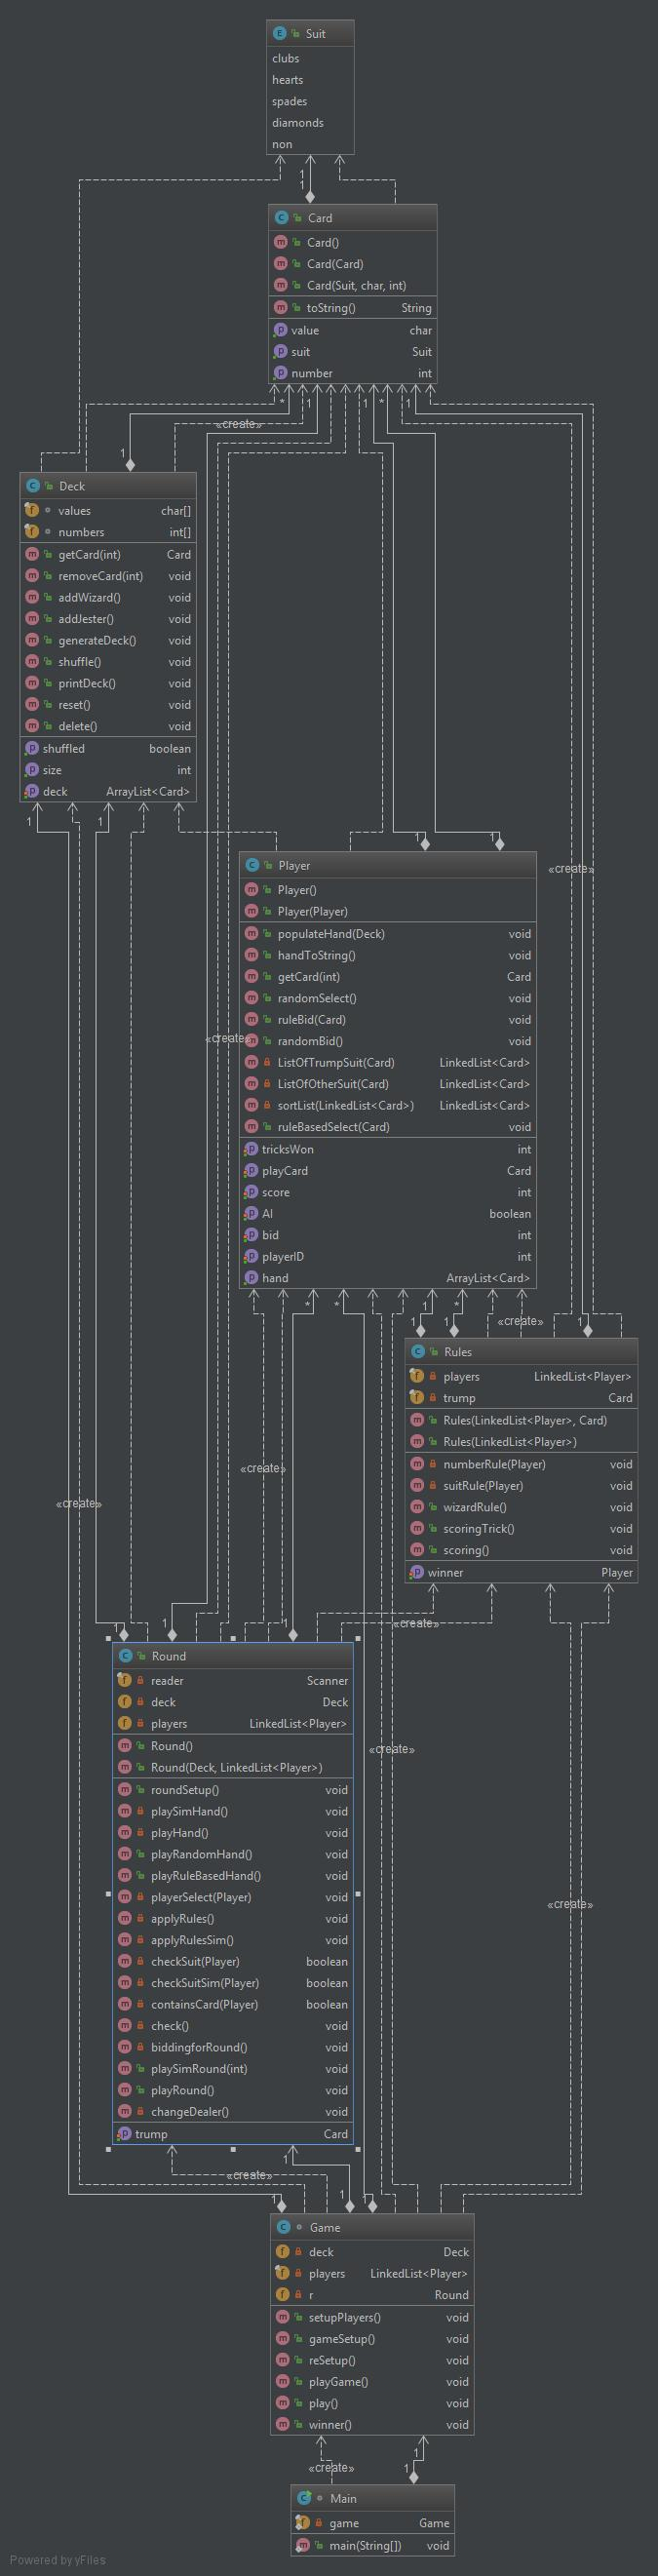
\includegraphics[width=15cm ,height=20cm,keepaspectratio]{Game_Classes}
\caption{Diagram Showing the Class Diagram of the Game Classes}
\end{figure}[h]
\paragraph{Card}
This Card class created Card objects that will contain variables for the suit, the value of the card in relation to the other and the number displayed on the card such as a wizards or an ace. It will also contain methods to construct the card and getters ans setters for each of the variables. Card will also contain a copying constructor for the use of the AI. This class wil mainly be used in the generation of the deck but will also be used in the sel
\paragraph{Deck}
Deck is a class for create a deck object to be used in the 
\paragraph{Player}
\paragraph{Round}
\paragraph{Rules}
\paragraph{Game}
\paragraph{Suit}
\paragraph{Main}
\subsubsection{Aritifical Intelligence Classes}
\begin{figure}[h]
\centering
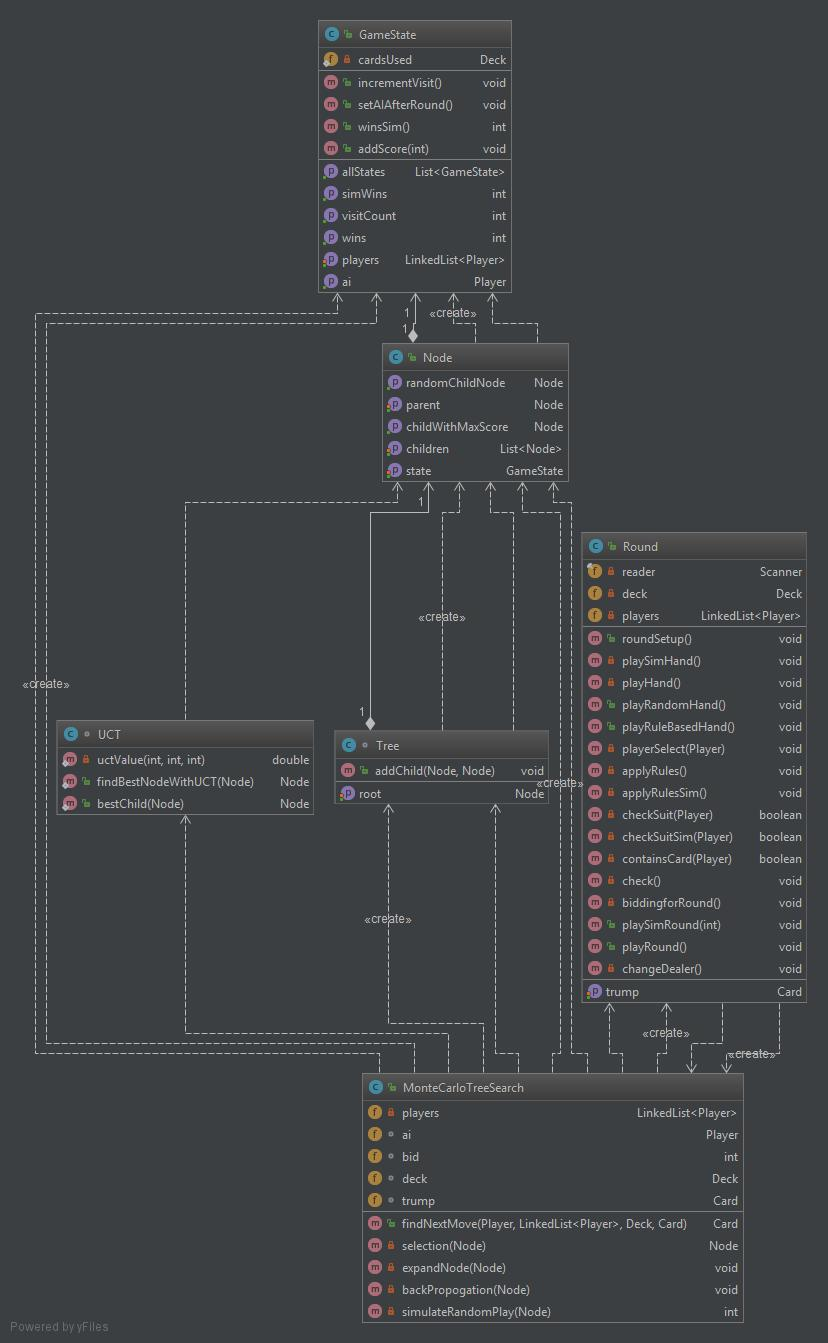
\includegraphics[width=15cm ,height=20cm,keepaspectratio]{AI_Classes}
\caption{Diagram Showing the Class Diagram of the AI Classes and the linking Round Class}
\end{figure}[h]
This section will show you the classes associated with Monte Carlo Tree Search AI. 
\paragraph{Node}

\paragraph{Tree}
\paragraph{GameState}
\paragraph{MonteCarloTreeSearch}
\paragraph{UCT}

\subsection{Data Flow Diagrams}
\section{Some detailed design}
In this section I will outline the important Algorithms to be used in the program and discuss how the User interface will looked and function.
\subsection{Algorithm Design}
\section{User Interface}
As this project is mainly based on the Artificial Intelligence, only a simple User interface is needed. So, using a Terminal UI seems the best choice. This will include showing the cards that the player has in their hand and the card they will play. This interface will also allow you to bid at the beginning of the round after the trump card and hands have been given out. After the round has been completed it shows the number of tricks that has been won, the score they have received based on their bid and trick they have won.
\section{Other relevant sections}

You should concentrate on the more important aspects of the design. It is essential that an overview is presented before going into detail. As well as describing the design adopted it must also explain what other designs were considered and why they were rejected.

The design should describe what you expected to do, and might also explain areas that you had to revise after some investigation.

Typically, for an object-oriented design, the discussion will focus on the choice of objects and classes and the allocation of methods to classes. The use made of reusable components should be described and their source referenced. Particularly important decisions concerning data structures usually affect the architecture of a system and so should be described here.

How much material you include on detailed design and implementation will depend very much on the nature of the project. It should not be padded out. Think about the significant aspects of your system. For example, describe the design of the user interface if it is a critical aspect of your system, or provide detail about methods and data structures that are not trivial. Do not spend time on long lists of trivial items and repetitive descriptions. If in doubt about what is appropriate, speak to your supervisor.
 
You should also identify any support tools that you used. You should discuss your choice of implementation tools - programming language, compilers, database management system, program development environment, etc.

Some example sub-sections may be as follows, but the specific sections are for you to define. 
